\documentclass[tikz,border=3pt]{standalone}
\usetikzlibrary{positioning,arrows.meta,shapes.geometric,backgrounds}

\begin{document}

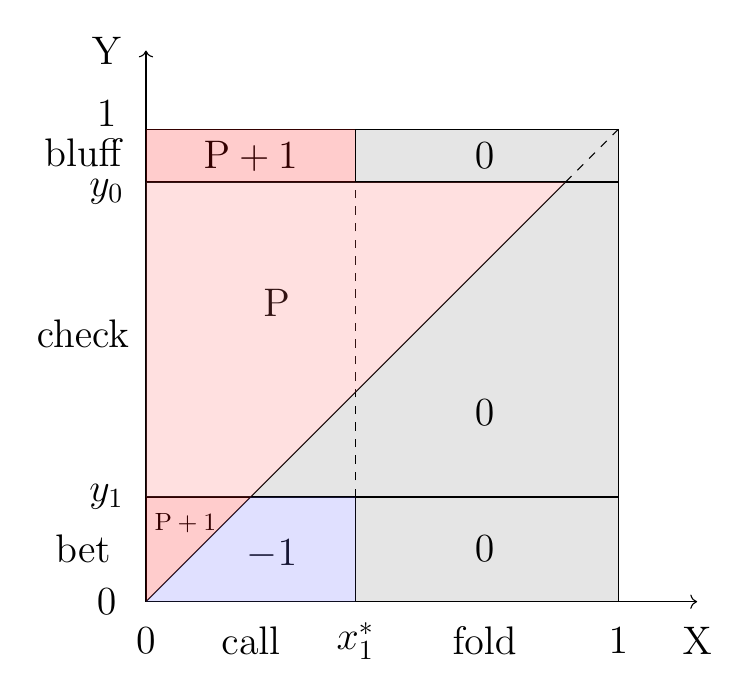
\begin{tikzpicture}

%%% 定型（編集あり）
\draw[->] (0,0) --(0,7);
\draw[->] (0,0) --(7,0);
\draw (0,6) --(6,6) --(6,0);

\node[font=\Large] at (7,-0.5) {X};
\node[font=\Large] at (-0.5,7) {Y};

\node[font=\Large] at (0,-0.5) {$0$};
\node[font=\Large] at (6,-0.5) {$1$};
\node[font=\Large] at (-0.5,0) {$0$};
\node[font=\Large] at (-0.5,6.2) {$1$};
%%%

%% 定数
%\pgfmathsetmacro{\y0}{5.33}

%% 線
\draw (0,5.33) --(6,5.33);
\draw (0,1.33) --(6,1.33);
\draw (2.66,0) --(2.66,1.33);
\draw[dashed] (2.66,1.33) --(2.66,5.33);
\draw (2.66,5.33) --(2.66,6);

\draw (0,0) --(5.33,5.33);
\draw[dashed] (5.33,5.33) --(6,6);


%% 目盛り
\node[font=\Large] at (2.66,-0.5) {$x_1^*$};
\node[font=\Large] at (-0.5,1.33) {$y_1$};
\node[font=\Large] at (-0.5,5.2) {$y_0$};

%% 数字
\node[font=\Large] at (1.33,5.66) {$\mathrm{P}+1$};
\node[font=\Large] at (1.66,3.8) {$\mathrm{P}$};
\node[font=\Large] at (4.3,5.66) {$0$};
\node[font=\Large] at (4.3,2.4) {$0$};
\node[font=\Large] at (4.3,0.67) {$0$};
\node[font=\Large] at (1.6,0.6) {$-1$};
\node[font=\small] at (0.5,1) {$\mathrm{P}+1$};

%% 範囲説明
% X axis
\node[font=\Large] at (1.33,-0.5) {call};
\node[font=\Large] at (4.3,-0.5) {fold};
% Y axis
\node[font=\Large] at (-0.8,3.4) {check};
\node[font=\Large] at (-0.8,0.67) {bet};
\node[font=\Large] at (-0.8,5.7) {bluff};

%% 色塗り
\fill[black, opacity=0.1] (2.66,0) rectangle (6,1.33);
\fill[black, opacity=0.1] (1.33,1.33) --(6,1.33) --(6,5.33) --(5.33,5.33) --cycle;
\fill[black, opacity=0.1] (2.66,5.33) rectangle (6,6);

\fill[red!60, opacity=0.2] (0,1.33) --(1.33,1.33) --(5.33,5.33) --(0,5.33) --cycle;
\fill[red, opacity=0.2] (0,0) --(1.33,1.33) --(0,1.33) --cycle;
\fill[red, opacity=0.2] (0,5.33) --(2.66,5.33) --(2.66,6) --(0,6) --cycle;

\fill[blue!60, opacity=0.2] (0,0) --(2.66,0) --(2.66,1.33) --(1.33,1.33) --cycle;

\end{tikzpicture}
\end{document}
